\documentclass[12pt,a4paper]{article}
\usepackage{graphicx}
\usepackage[applemac]{inputenc} %% european characters can be used (Mac OS)
% ------------------------------------------------
\usepackage[T1]{fontenc}   %% get hyphenation and accented letters right
\usepackage{mathptmx}      %% use fitting times fonts also in formulas
\pagestyle{empty}                %% no page numbers!
\usepackage[left=35mm, right=35mm, top=15mm, bottom=20mm, noheadfoot]{geometry}

% begin the document
\begin{document}
\thispagestyle{empty}

\title{\textbf{When a Plant Disease Epidemiologist works with data science}}
\author{Sith Jaisong \\
Plant Disease Management Group, CESD, IRRI\\ Los Ba\~{n}os, Philippines\\
s.jaisong@irri.org}
\date{} % <--- leave date empty
\maketitle\thispagestyle{empty} %% <-- you need this for the first page
% introduction should have the objective or the problem or even telling the reader what you wanna say, and 

% I'd like you to follow the American Phytopathological Society guidelines for abstract submission

%Presentation Title
%Capitalize only the first letter of the first word and any proper nouns, (e.g., Effect of pesticides on recovery of Didymella bryoniae from cucurbit vines). The title is limited to 150 characters including spaces. (Approximately 30 word count.) Registered names and trademarks are not permitted in title.
%
%
%
%Abstract Text
%Read the technical requirements and view the sample abstract before submitting your abstract.
%
%The abstract must be in one paragraph.
%DO NOT include the title, author name(s), or author affiliations in the abstract text field.
%Copy the abstract and paste it into the submission form abstract text box under the Abstract Copy/Body field header.
%Or type text in to the abstract field.
%Use the abstract toolbar to add formatting (italics, superscripts, subscripts, Greek or math symbols), or use the start coding <i> and the stop coding </i>, if you prefer.
%If the symbol is not available, spell it out (e.g., theta).
%Character limit is 1,490 characters including spaces (Approximately 250 word count).
%
%
%Sample Abstract
%Didymella bryoniae, the fungus that causes gummy stem blight, survives between crops in cucurbit debris. A pesticide that eliminates the fungus from infested debris would reduce initial inoculum for subsequent crops planted in infested fields. Naturally infected, 5-cm muskmelon vine sections were sprayed with field-equivalent rates of three herbicides, four fungicides, six salts, three botanical extracts, or three organic pesticides. After 3 days, vine sections were cut into 1-cm pieces and cultured on 1/4 PDA plus antibiotics. Each pesticide was tested 2 to 4 times with 10 to 20 vine sections per treatment. Chlorothalonil, mancozeb, sodium bisulfite, and pyraclostrobin + boscalid (Pristine) consistently reduced recovery of D. bryoniae to an average of 63, 57, 41, and 8% of vine pieces, respectively, compared to a water-treated control (99%). The other pesticides did not significantly reduce recovery of the fungus. Using Pristine to treat debris at the end of the season is not advisable, because of the risk of resistance to this fungicide. However, a non-specific material, such as a broad-spectrum fungicide or a salt, could be used to reduce the amount of surviving inoculum.


% Further comments on the abstract
% No citations in abstracts
% No figures in abstracts

% What is "data science"? That would be the best first sentence or two to orient us.
% Your last five sentences really need to be part of the whole abstract. Integrate the processes don't separate Data Science and epidemiology here. Illustrate the frameworks in tandem, don't make them two parts. The way it reads now, it's redundant.

Data generally are raw and need to be cleaned in order to extract meaning from them or solve the problems. There are many methods in data processing that botanic epidemiology can borrow from data science. Epidemiologists often deal with more than one factor possibly causing or contributing to plant disease. Temperature, moisture, soil pH, soil type, plant varieties, crop density are some examples of variables considering the causes of plant disease development. When this number of variables are added to a study, the dataset becomes massive and requires powerful tools to manage it. Data science is emerging to meet the challenge of processing very large data. It applies techniques from statistics and computer science, extracting the meaning from the data and produce graphs, models, and other representations of the data, etc. in order to answer questions. The process starts with collecting the data that are able to answer the questions or hypothesis. Joining, combining, or wrangling the data are the processes after collection. In reality data may need to be cleaned (outlier and missing value removal or imputation). Once we have a clean dataset, exploratory data analysis may be applied. Next, designing models by using an algorithm such as k-nearest neighbor (k-NN), linear regression etc. may be used. The model selected depends upon the type of questions being asked. Then, we can interpret, visualize, report or communicate the result. The process of data science is in common with plant disease epidemiology. Epidemiologists often deal with more than one variable possibly causing the plant disease. Plant diseases develop from interaction between plant and its pathogen but also environment (weather) and human activities referring to the agricultural practices. The models are effective features capturing these relationships. They are developed for many uses or objectives. The most common ones are description, understating, prediction, comparison, and communication.The ideas and the process of tackling the problem are in the same concept. Therefore, data science process is the promising framework that epidemiologist should have in mind.

%\begin{figure}[h!]
%%uncomment next line to include a graphic file
%\centerline{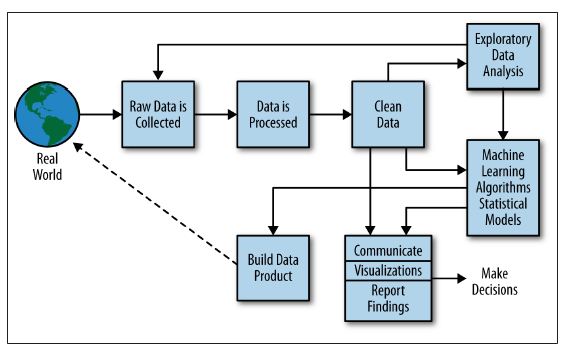
\includegraphics[width=8cm]{Figure2-2}}
%%and comment out next line
%%\centerline{\framebox[6cm]{\rule{0cm}{3.5cm} figure example}}
%\caption{Data science process \cite{schutt2013doing}}
%\label{fig1}
%\end{figure}

\bibliography{seminar}
\bibliographystyle{plain}
\end{document}